\documentclass{beamer}


\usepackage{animate}
\usepackage[spanish]{babel}
\usepackage[utf8]{inputenc}
\usepackage{amsmath}
\usepackage{pgfplots}
 \usepackage{graphicx}
\usetheme{Madrid}
\title{Método de Newton-Raphson y la secante}

\author{H.D Salinas, Bing \\
Curso de métodos computacionales\\
Universidad de Antioquia\\}


\date{\today}

\begin{document}

\begin{frame}
  \titlepage
\end{frame}

\begin{frame}{Metodo }
  Sea $f$ una función real derivable en un intervalo abierto que contiene una raíz $\alpha$, es decir, $f(\alpha)=0$. Queremos encontrar una aproximación de $\alpha$ usando el método de Newton-Raphson.

Para ello, partimos de un valor inicial $x_0$ cercano a $\alpha$ y aplicamos la fórmula recursiva:
\[x_{n+1}=x_n-\frac{f(x_n)}{f'(x_n)}, \quad n=0,1,2,\dots\]
\end{frame}

\begin{frame}{Deducción del método}
¿Cómo se obtiene esta fórmula? Usando la expansión en serie de Taylor de $f$ alrededor de $x_n$, tenemos que:
\pause
\[f(x)=f(x_n)+f'(x_n)(x-x_n)+\frac{f''(\xi)}{2}(x-x_n)^2,\]
donde $\xi$ es un punto entre $x$ y $x_n$. Si hacemos 
$x=\alpha$, obtenemos:
\pause
\[0=f(\alpha)=f(x_n)+f'(x_n)(\alpha-x_n)+\frac{f''(\xi)}{2}(\alpha-x_n)^2.\]
\pause
Despejando $\alpha$, tenemos que:
\[\alpha=x_n-\frac{f(x_n)}{f'(x_n)}-\frac{f''(\xi)}{2 f'(x_n)}(\alpha-x_n)^2.\]
\end{frame}

\begin{frame}{Deducción del método (cont.)}
Si el valor inicial $x_0$ es suficientemente cercano a $\alpha$, podemos suponer que los términos $(\alpha-x_0)$ y $(\alpha-x_1)$ son pequeños y por tanto el último término de la ecuación anterior es despreciable. Así, obtenemos una aproximación lineal de $\alpha$:
\[\alpha \approx x_1=x_0-\frac{f(x_0)}{f'(x_0)}.\]
Repetiendo este proceso con el nuevo valor $x_1$, obtenemos otra aproximación mejorada:
\[\alpha \approx x_2=x_1-\frac{f(x_1)}{f'(x_1)},\]
y así sucesivamente. De esta forma, generamos una sucesión $\{x_n\}$ que converge a la raíz $\alpha$ siempre que se cumplan ciertas condiciones sobre la función $f$ y el valor inicial $x_0$. Este es el método de Newton-Raphson.
  
\end {frame}



  
\begin{frame}{Interpretación Geométrica}
\begin{figure} 
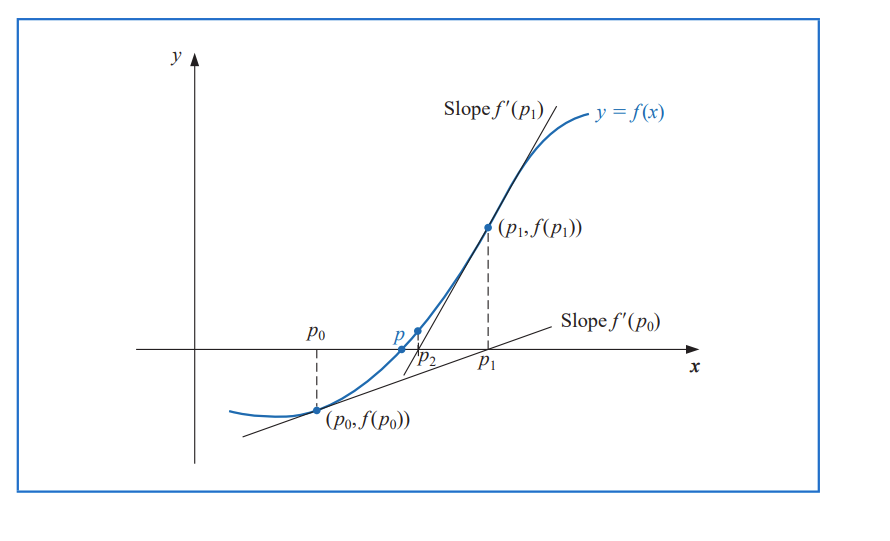
\includegraphics[width=0.7\textwidth]{NewtonRaphsod.png} \caption{Interpretacion Gemétrica.} \end{figure} 
\end{frame}




\begin{frame}{Ejemplo de oscilación} 

\begin{itemize}

\item Un ejemplo donde el método de Newton-Raphson se queda oscilando sin llegar a la raíz es cuando se aplica a la función \[f(x) = x^3 - 2x + 2.\] 

\item Esta función tiene una única raíz real en $x \approx -1.7693$. Sin embargo, si se elige un valor inicial $x_0 = 0$, 

\item  El método puede converger a un mínimo o máximo local en lugar de al mínimo o máximo global, lo que puede llevar a una estimación incorrecta de la raíz.

\item El método no converge a la raíz sino que salta entre dos valores alternos: $x_1 = -1$ y $x_2 = 1$. Esto se debe a que la derivada de la función en esos puntos es cero, lo que hace que el método falle. 
 
 \end{itemize} 

 \end{frame}





\begin{frame}{Ejemplo de oscilación} 
   \begin{center}
     \scalebox{1.0}{
    \begin{tikzpicture}
      \begin{axis}[
        xlabel=$x$,
        ylabel=$y$,
        xmin=-5,
        xmax=5,
        ymin=-5.1,
        ymax=5.1
      ]
      \addplot[blue,samples=100] {x^3-2*x+2};
      \addplot[mark=*] coordinates {(-1.7693,0)};
      \addplot[mark=*] coordinates {(0,2)};
      \addplot[red,samples=100] {-2*x+2};
      \addplot[mark=*] coordinates {(1.,0)};      
      \addplot[dashed] coordinates {(0,-5) (0,5)};
      \addplot[dashed] coordinates {(-5,0) (5,0)};
      \end{axis}
    \end{tikzpicture}}
  \end{center}
\end{frame}



\begin{frame}{Ejemplo de oscilación} 
   \begin{center}
     \scalebox{1.0}{
    \begin{tikzpicture}
      \begin{axis}[
        xlabel=$x$,
        ylabel=$y$,
        xmin=-5,
        xmax=5,
        ymin=-5.1,
        ymax=5.1
      ]
      \addplot[blue,samples=100] {x^3-2*x+2};
      \addplot[mark=*] coordinates {(-1.7693,0)};
      \addplot[mark=*] coordinates {(0,2)};          
      \addplot[dashed] coordinates {(0,-5) (0,5)};
      \addplot[dashed] coordinates {(-5,0) (5,0)};      
      \addplot[mark=*] coordinates {(1.,1)};  
      \addplot[mark=*] coordinates {(0.,0)};  
      \addplot[red, samples=100] {x};
      \end{axis}
    \end{tikzpicture}}
  \end{center}
\end{frame}






\begin{frame}{Ejemplos de errores} \begin{enumerate} 

\item El método puede no converger si la estimación inicial está demasiado lejos de la raíz verdadera. Por ejemplo, si se aplica el método a la función

\[f(x) = e^{-x} - x,\] 

que tiene una única raíz real en 
$ x \approx 0.5671 $,  y se elige un valor inicial $x_0 \approx -10$, el método diverge y los valores obtenidos se alejan cada vez más de la raíz. 



\end{enumerate}
    \begin{center}
     \scalebox{0.5}{
    \begin{tikzpicture}
      \begin{axis}[
        xlabel=$x$,
        ylabel=$y$,
        xmin=-5,
        xmax=5,
        ymin=-1.1,
        ymax=1.1
      ]
      \addplot[blue,samples=100] {exp(-x)-x};
      \end{axis}
    \end{tikzpicture}}
  \end{center}

\end{frame}


\begin{frame}{Deducción del método de la secante}
  El metodo de Newton tiene una debilidad y es la necesidad de 
   conocer la derivada. Una variante del metodo es el metodo de la secante:
   
  Empezamos con la serie de Taylor de una función $f(x)$ alrededor de un punto $x_0$:
  \pause
  $$f(x) = f(x_0) + f'(x_0)(x-x_0) + \frac{f''(x_0)}{2!}(x-x_0)^2 + \cdots$$
  \pause
  Si tomamos dos puntos cercanos a una raíz de la función, $x_n$ y $x_{n-1}$, podemos aproximar la función por una recta secante que pasa por esos puntos empleando una aproximación con la definición de la derivada,  $f'(x_0)$  :
  \pause
  $$f(x) \approx f(x_n) + \frac{f(x_n)-f(x_{n-1})}{x_n-x_{n-1}}(x-x_n)$$
  \pause
  Si igualamos esta expresión a cero y despejamos $x$, obtenemos la siguiente fórmula para el siguiente punto de la iteración:
  \pause
  $$x_{n+1} = x_n - \frac{f(x_n)(x_n-x_{n-1})}{f(x_n)-f(x_{n-1})}$$
  
  Este es el método de la secante para encontrar ceros de una función.
\end{frame}

\begin{frame}{Interpretación geométrica}
    \begin{figure} 
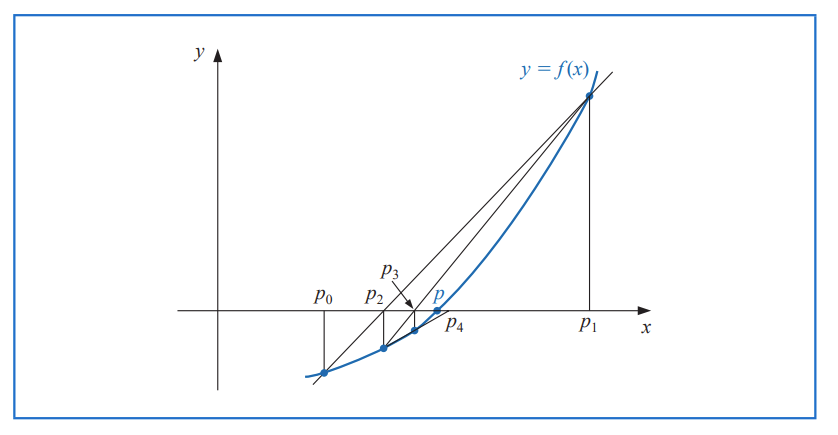
\includegraphics[width=0.7\textwidth]{secante.png} \caption{Interpretacion Gemétrica.} \end{figure} 
\end{frame}


\begin{frame}{Función que no se puede aplicar el método de la secante}
\begin{itemize}
\item $f(x)=\sin(x^2)$. Esta función tiene un comportamiento oscilatorio y irregular.

\item Si los valores iniciales están muy lejos de la raíz o si son muy cercanos entre sí, el método de la secante puede ser divergente o lento. 
  
\end{itemize}
    \begin{center}
     \scalebox{0.9}{
    \begin{tikzpicture}
      \begin{axis}[
        xlabel=$x$,
        ylabel=$y$,
        xmin=-5,
        xmax=5,
        ymin=-1.1,
        ymax=1.1
      ]
      \addplot[blue,samples=100] {sin(deg(x^2))};
      \end{axis}
    \end{tikzpicture}}
  \end{center}

\end{frame}






\begin{frame}{Errores del método de la secante}
  Los errores del método de la secante son los siguientes:  
  \begin{itemize}
    \item El método de la secante puede ser \textbf{divergente}, es decir, que no garantiza que se encuentre una raíz de la función.
    
    \item El método de la secante tiene un orden de convergencia menor que el método de Newton-Raphson, que usa la derivada exacta de la función. Esto significa que el método de la secante necesita más \textbf{iteraciones} para alcanzar una precisión deseada.
    
    \item El método de la secante requiere dos valores iniciales, que pueden ser difíciles de escoger si no se conoce el comportamiento de la función o el intervalo donde se encuentra la raíz. Además, estos valores deben ser distintos entre sí y no deben anular el denominador de la fórmula del método.
  \end{itemize}
\end{frame}

\begin{frame}{Errores del método de la secante}
\begin{itemize}
\item La función es constante o tiene una derivada nula en el punto buscado.
\item La función tiene un punto de inflexión en el punto buscado.
\item La función tiene una asíntota vertical cerca del punto buscado.

\item Los valores iniciales son muy lejanos al punto buscado o están en regiones donde la función cambia bruscamente.

\end{itemize}
\end{frame}




\begin{frame}{Referencias}
\begin{itemize}
 \item Burden, R. L., Faires, J. D., & Burden, A. M. (2016). Análisis numérico (10a ed.). Cengage Learning.3

\item 

\begin{figure} 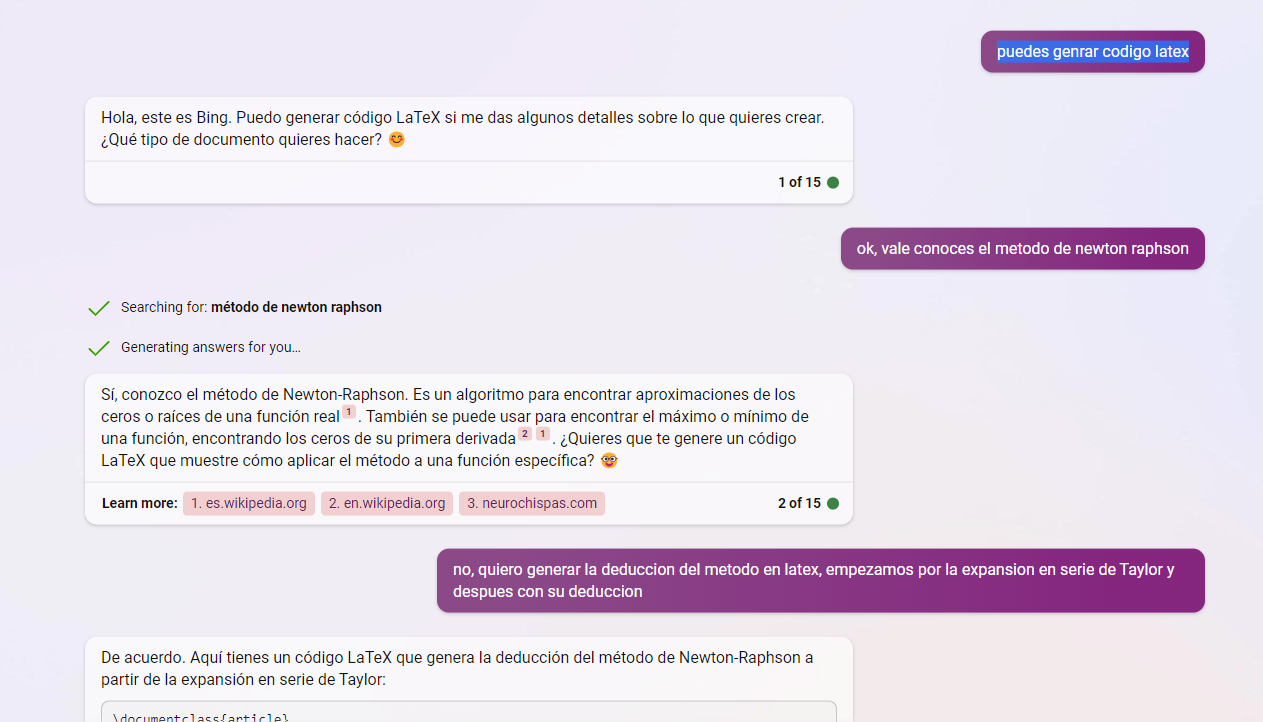
\includegraphics[width=0.7\textwidth]{prompts-de-beam.png} \caption{Prompts de bing.} \end{figure} 

\end{itemize}
\end{frame}

 \end {document}


 